\documentclass[10pt]{article}
\usepackage[utf8]{inputenc}
\usepackage[T1]{fontenc}
\usepackage{amsmath}
\usepackage{amsfonts}
\usepackage{amssymb}
\usepackage[version=4]{mhchem}
\usepackage{stmaryrd}
\usepackage{hyperref}
\hypersetup{colorlinks=true, linkcolor=blue, filecolor=magenta, urlcolor=cyan,}
\urlstyle{same}
\usepackage{mathrsfs}
\usepackage{graphicx}
\usepackage[export]{adjustbox}
\graphicspath{ {./images/} }
\usepackage{graphicx} % For including images
\usepackage{subcaption} % For subfigures

\usepackage{graphicx}

\title{The RK4 solution of SIR and SIS epidemic models}

\author{
    Roshan Kumar \\
    MA21BTECH11013
    \and
    Devashish Chaudhari \\
    MA21BTECH11005
}
    


\date{}


%New command to display footnote whose markers will always be hidden
\let\svthefootnote\thefootnote
\newcommand\blfootnotetext[1]{%
  \let\thefootnote\relax\footnote{#1}%
  \addtocounter{footnote}{-1}%
  \let\thefootnote\svthefootnote%
}

%Overriding the \footnotetext command to hide the marker if its value is `0`
\let\svfootnotetext\footnotetext
\renewcommand\footnotetext[2][?]{%
  \if\relax#1\relax%
    \ifnum\value{footnote}=0\blfootnotetext{#2}\else\svfootnotetext{#2}\fi%
  \else%
    \if?#1\ifnum\value{footnote}=0\blfootnotetext{#2}\else\svfootnotetext{#2}\fi%
    \else\svfootnotetext[#1]{#2}\fi%
  \fi
}

\begin{document}
\maketitle

\begin{flushright}
Source code: \href{https://github.com/Numerologists/Using-Numerical-Methods-in-Finding-Solutions-of-Epidemic-Models}{Github}
\end{flushright}

\begin{abstract}
In this paper, the SIR and SIS epidemic models in biology are solved using a numerical method, specifically the fourth-order Runge-Kutta (RK4) method, for handling nonlinear differential equations. Both the SIR and SIS models are represented by sets of coupled nonlinear differential equations. The RK4 method computes approximate numerical solutions by iteratively evaluating derivatives at several points within each integration step.

Our numerical approach yields results that closely match those obtained from analytic techniques. While our method utilizes numerical computation rather than explicit analytic series, it provides a robust means of solving these epidemic models and can be extended to tackle other systems of coupled nonlinear differential equations in biology.
\end{abstract}


\section*{1. History of Epidemics}
The history of epidemics reveals the profound impact of infectious diseases on human societies. Notable events include the 14th century Black Death in Europe, which drastically reduced the population, and the ancient Plague of Athens, described by Thucydides, whose exact nature remains debated.

Ancient perceptions of contagion often attributed epidemics to miasma or divine punishment, with limited understanding of person-to-person transmission until the 19th century. Epidemics like the Yellow Fever outbreak in 1793 and the 1918 influenza pandemic reshaped communities and healthcare.

Mathematical modeling of disease dynamics, pioneered by Bernoulli in 1760, has played a crucial role in assessing vaccination strategies and public health interventions. Today, globalization and drug resistance present complex challenges, underscoring the need for interdisciplinary collaboration and historical insight in combating infectious diseases.
\section*{2. Introduction}
Epidemiology is the branch of biology which deals with the mathematical modeling of spread of diseases. Many problems arising in epidemiology may be described, in a first formulation, by means of differential equations. This means that the models are constructed by averaging some population and keeping only the time variable. To the best of our knowledge the first mathematical model of epidemiology was formulated and solved by Daniel Bernoulli in 1760 . Since the time of Kermack and McKendrick [1], the study of mathematical epidemiology has grown rapidly, with a large variety of models having been formulated and applied to infectious diseases [2-4].

Unfortunately, sometimes even the simplest mathematical models of natural phenomena with sets of first-order ordinary differential equations are non-integrable. Nucci and Leach [5] have discussed these features and obtained an integrable SIS model by applying Lie analysis. Many other mathematical tools such as stability theory [6], bifurcation theory [7], Lyapunov method [8], Poincaré-Bendixson type theorems [9], index and topological concepts can be used to study these differential equations arising in biology. There is an extensive literature concerning SIR and SIS models. Considerable attention has been given to these models by several authors see [2-14]. As far as we know, there is no analytic solution of these models, as mentioned by Singh $[13]$.

Consider a population which remains constant and which is divide into three classes: the susceptibles, denoted by $S$, who can catch the disease; the infectives, denoted by $I$, who are infected and can transmit the disease to the susceptibles, and the removed class, denoted by $R$, who had the disease and recovered or died or have developed immunity or have been removed from contact with the other classes. Since from the modeling perspective only the overall state of a person with respect to the disease is relevant, the progress of individuals is schematically described by

$$
S \rightarrow I \rightarrow R
$$




These types of models are known as SIR models. This model is deterministic.

In the SIS model, the infectives, $I$, return to the susceptible class, $S$, on recovery because the disease confers no immunity against reinfection. Such models are more effective for diseases caused by bacteria or helminth agents and also for most sexually transmitted disease. The progress of individuals in this model is schematically described by

$$
S \rightarrow I \rightarrow S
$$

Kermack and McKendrick [1] provided the mathematical models for SIR and SIS.

In this paper, we will explore the application of RK4 to the analysis of the SIR and SIS models, focusing on generating numerical solutions that align with theoretical predictions and existing numerical results. Through this approach, we aim to validate the efficacy of RK4 in modeling epidemiological dynamics and providing insights into disease propagation and control strategies.


\section*{3. RK4 method for SIR model}

\vspace{2\baselineskip}
Given the SIR model equations:
\begin{align*}
\frac{ds}{dt} &= -r s(t) i(t), \\
\frac{di}{dt} &= r s(t) i(t) - \alpha i(t),
\end{align*}
with initial conditions \(s(0) = S_0>0\) and \(i(0) = I_0>0\).

To use RK4, we will discretize time \(t\) into small steps of size \(h\). The RK4 method uses weighted averages of derivatives at different points within each time step to approximate the solution. Here is how to implement RK4 for the SIR model:

Define the Initial Conditions and Parameters:
\begin{itemize}
    \item \(S_0\) = initial number of susceptible individuals
    \item \(I_0\) = initial number of infectious individuals
    \item \(s(t)\)=number of susceptible individuals
    \item \(i(t)\)=number of infectives individuals
    \item \(r\) = susceptivity coefficient
    \item \(\alpha\) = infectivity recovered coefficient
    \item \(h\) = time step
    
\end{itemize}

Implement RK4:
\begin{align*}
k_{1s} &= -r s_n i_n, & k_{1i} &= r s_n i_n - \alpha i_n, \\
k_{2s} &= -r \left(s_n + \frac{h}{2} k_{1s}\right) \left(i_n + \frac{h}{2} k_{1i}\right), & k_{2i} &= r \left(s_n + \frac{h}{2} k_{1s}\right) \left(i_n + \frac{h}{2} k_{1i}\right) - \alpha \left(i_n + \frac{h}{2} k_{1i}\right), \\
k_{3s} &= -r \left(s_n + \frac{h}{2} k_{2s}\right) \left(i_n + \frac{h}{2} k_{2i}\right), & k_{3i} &= r \left(s_n + \frac{h}{2} k_{2s}\right) \left(i_n + \frac{h}{2} k_{2i}\right) - \alpha \left(i_n + \frac{h}{2} k_{2i}\right), \\
k_{4s} &= -r \left(s_n + h k_{3s}\right) \left(i_n + h k_{3i}\right), & k_{4i} &= r \left(s_n + h k_{3s}\right) \left(i_n + h k_{3i}\right) - \alpha \left(i_n + h k_{3i}\right),
\end{align*}
where \(s_n\) and \(i_n\) represent the values of \(s\) and \(i\) at time \(t_n\).

Update the values of \(s\) and \(i\) for the next time step:
\begin{align*}
s_{n+1} &= s_n + \frac{h}{6} (k_{1s} + 2k_{2s} + 2k_{3s} + k_{4s}), \\
i_{n+1} &= i_n + \frac{h}{6} (k_{1i} + 2k_{2i} + 2k_{3i} + k_{4i}).
\end{align*}

Iterate the above calculations for each time step \(n = 0, 1, 2, \dots\) until the desired endpoint is reached.
  The classic SIR model [1] is described by




Let us write

$$
I_{\infty}=i(+\infty), \quad S_{\infty}=s(+\infty)
$$

It is known from the  publications (mentioned in paper)  that $i(t)$ decreases monotonously from $I_{0}$ to 0 when $r S_{0} / \alpha<1$. However, in case of $r S_{0} / \alpha>1, i(t)$ first increases to the maximum value and then decreases to zero. Thus, it always holds $I_{\infty}=0$.
\newline

Now lets verify with RK4\_method.


\begin{figure}[!htbp]
  \centering
  \subfloat[\(rS_0 > \alpha\)]{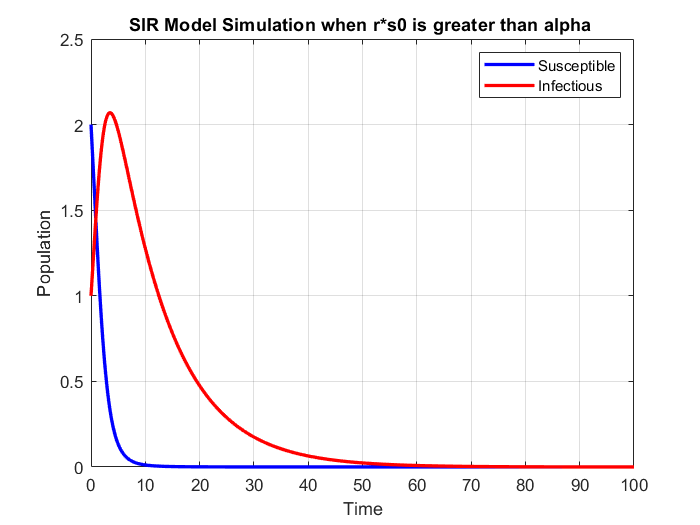
\includegraphics[width=0.5\textwidth]{images/when_rs0_is_greater_than_alpha.png}\label{fig:f1}}
  \hfill
  \subfloat[\(rS_0 < \alpha\)]{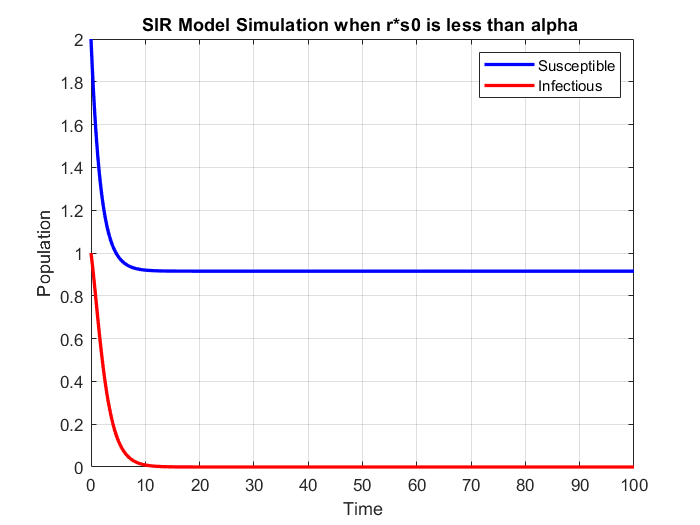
\includegraphics[width=0.5\textwidth]{images/when_rs0_is_less_than_alpha.png}\label{fig:f2}}
  \caption{Comparison of two cases based on \(rS_0\) and \(\alpha\) }
\end{figure}
   
\subsection*{2.1. Solution analysis of the SIR model with examples}
Let's define the threshold quantity $R_{0}=\frac{S_{0} r}{\alpha}$. It is assumed that $s^{\prime}<0$ for all $t$ and $i^{\prime}>0$ when $R_{0}>1$. This means $I$ will initially increase to some maximum if $R_{0}>1$, but eventually decreases and approaches zero, since $S$ is always decreasing. Our RK4 solution for the SIR model provides results that agrees with this  qualitative analysis given in paper.

The case with $R_{0}>1$ is of interest as it indicates epidemic. For $R_{0}<1, I$ will simply goes to zero, indicating no epidemic. 

\vspace{2\baselineskip}
 Example $1: \alpha=2, r=1 / 5, I_{0}=25, S_{0}=75$


In this case, we have $r S_{0} / \alpha=7.5>1, S_{\infty}=0, \beta=2$. 

\begin{figure}[!htbp]
  \centering
  \subfloat[paper\_result]{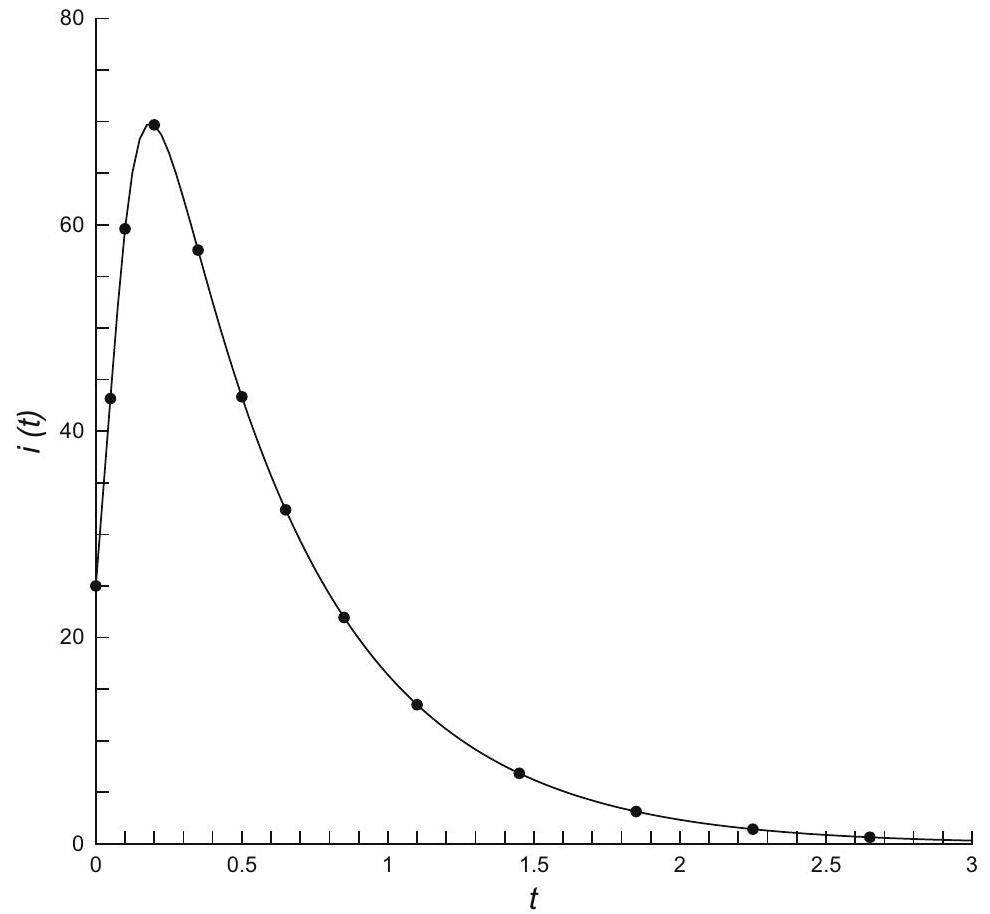
\includegraphics[width=0.5\textwidth]{2024_05_06_fa20b94a24cdaf499645g-07(1)}\label{fig:paper_11}}
  \hfill
  \subfloat[own\_result]{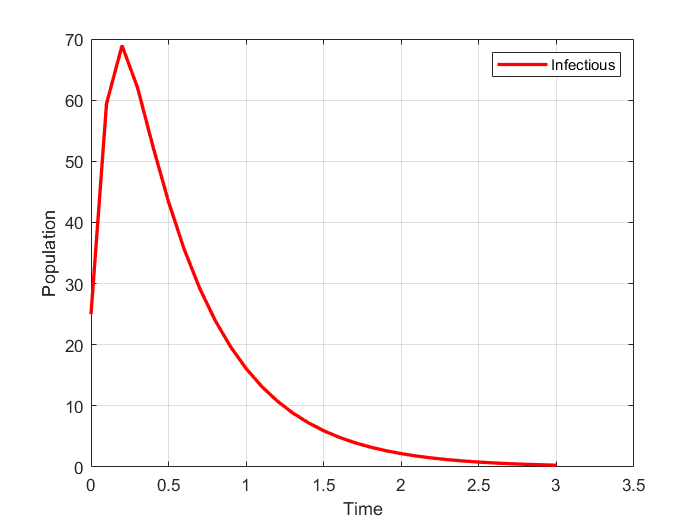
\includegraphics[width=0.5\textwidth]{images/exmple_2.png}\label{fig:RK4_11}}
  \caption{Comparison of \(I\) values obtained from the paper's results with our own results  }
\end{figure}
\begin{figure}[!htbp]
  \centering
  \subfloat[paper\_result]{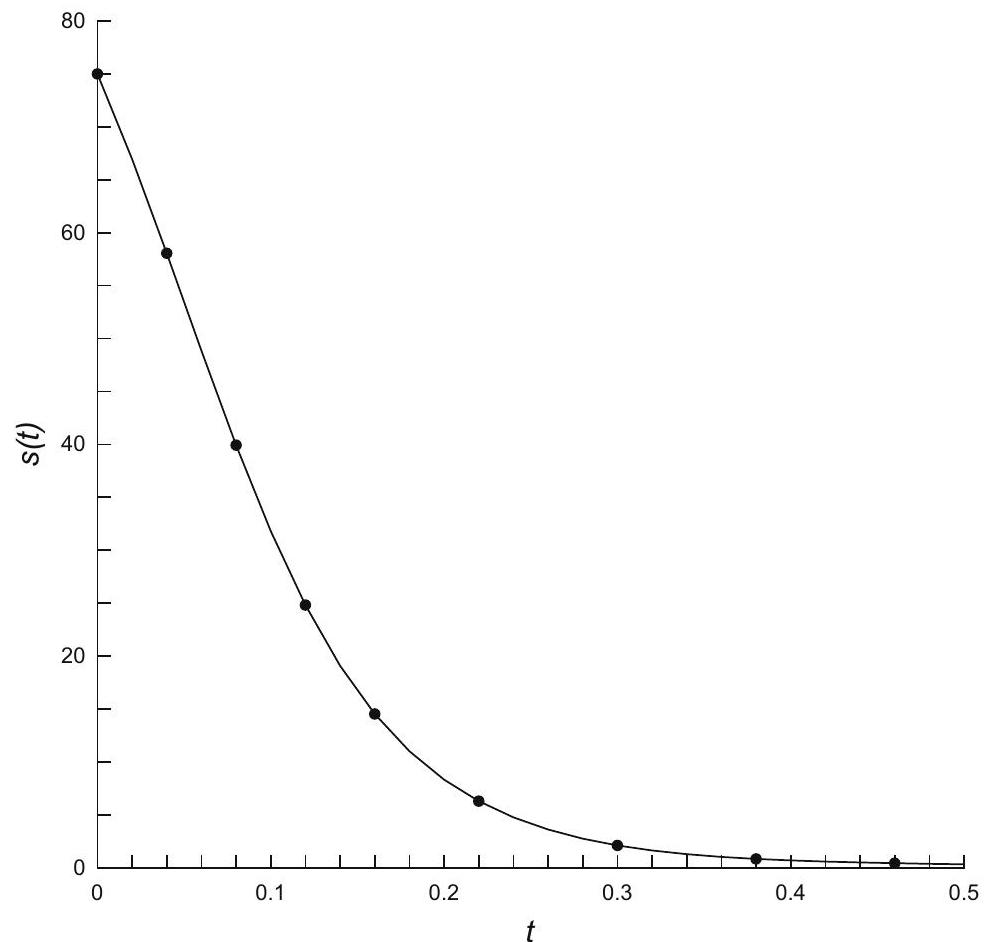
\includegraphics[width=0.5\textwidth]{images/2024_05_06_fa20b94a24cdaf499645g-07.jpg}\label{fig:paper_12}}
  \hfill
  \subfloat[own\_result]{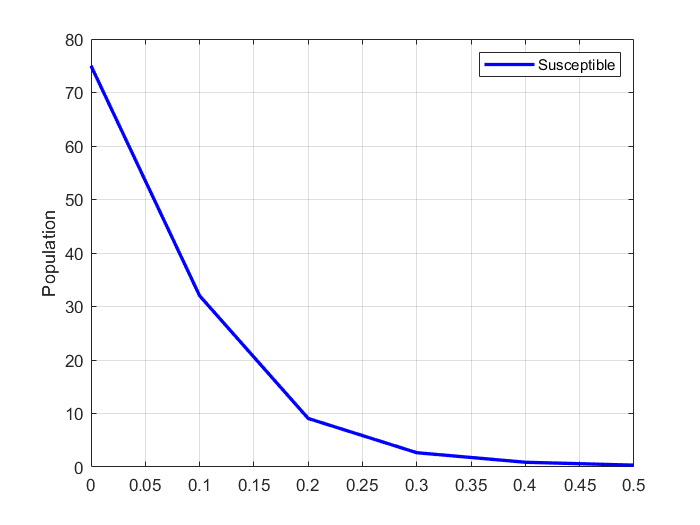
\includegraphics[width=0.5\textwidth]{images/fig_3.png}\label{fig:RK4_12}}
  \caption{Comparison of \(S\) values obtained from the paper's results with our own results  }
\end{figure}
\newpage
 Example 2: $\alpha=3 / 2, r=1 / 10, I_{0}=10, S_{0}=50$

In this case, we have $r S_{0} / \alpha=3.333>1, S_{\infty}=0.97, \beta=1.403$. 
\begin{figure}[!htbp]
  \centering
  \subfloat[paper\_result]{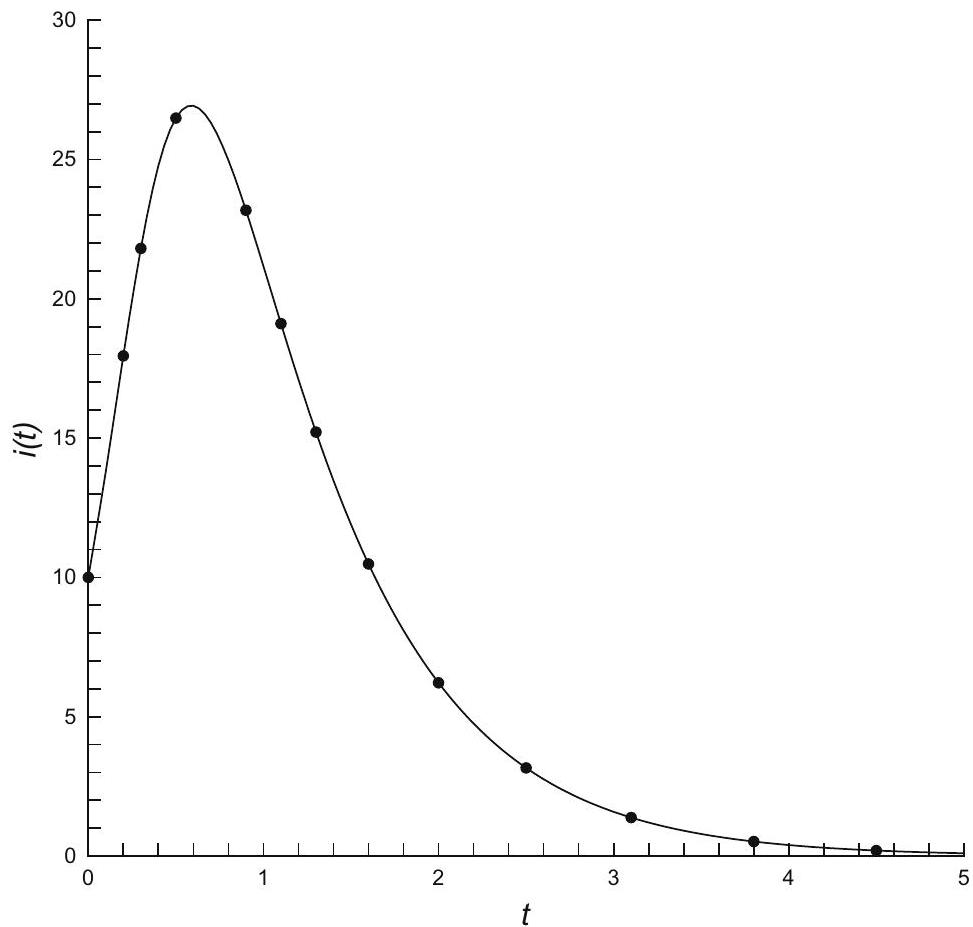
\includegraphics[width=0.5\textwidth]{images/2024_05_06_fa20b94a24cdaf499645g-08.jpg}\label{fig:paper_21}}
  \hfill
  \subfloat[own\_result]{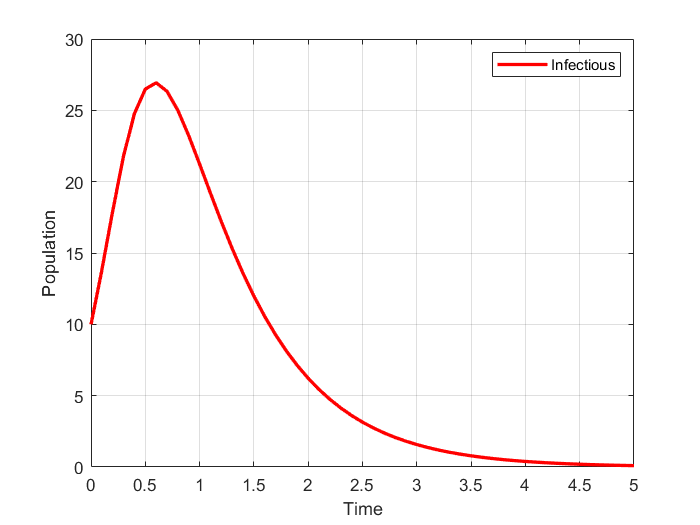
\includegraphics[width=0.5\textwidth]{images/fig_4.png}\label{fig:RK4_21}}
  \caption{Comparison of \(I\) values obtained from the paper's results with our own results  }
\end{figure}
\begin{figure}[!htbp]
  \centering
  \subfloat[paper\_result]{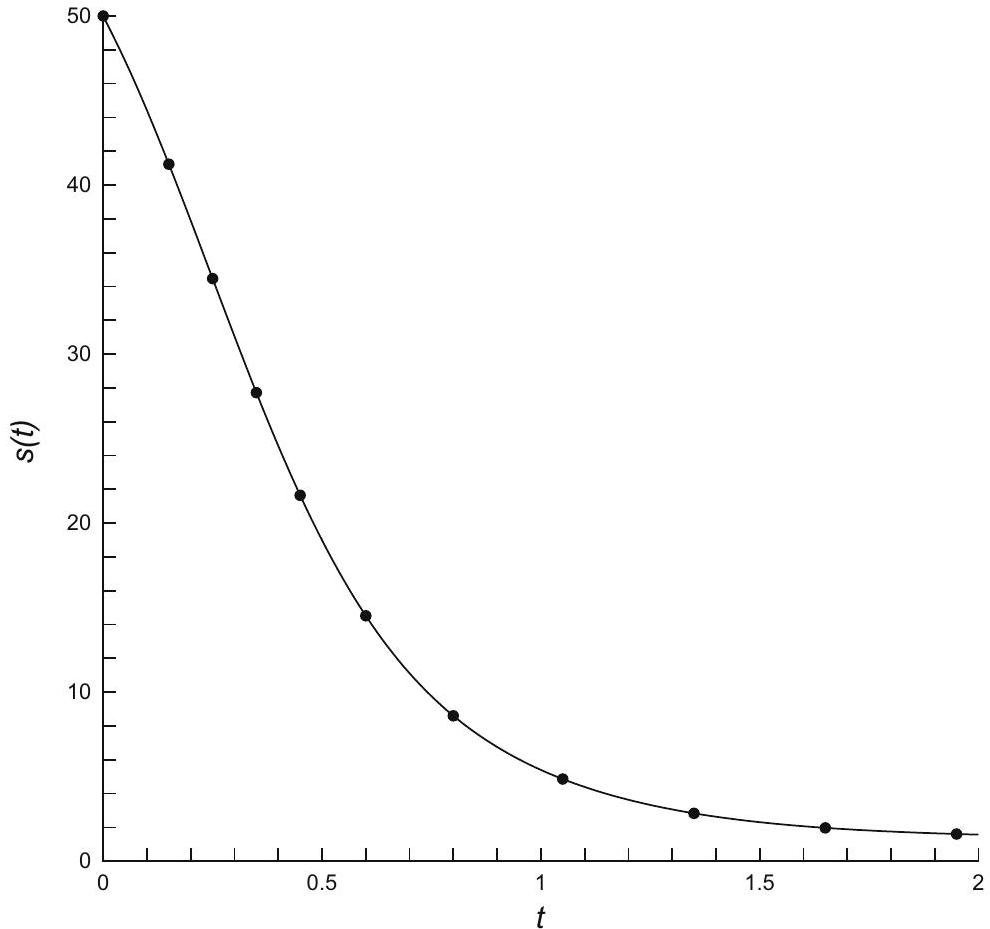
\includegraphics[width=0.5\textwidth]{images/2024_05_06_fa20b94a24cdaf499645g-08(1)}\label{fig:paper_22}}
  \hfill
  \subfloat[own\_result]{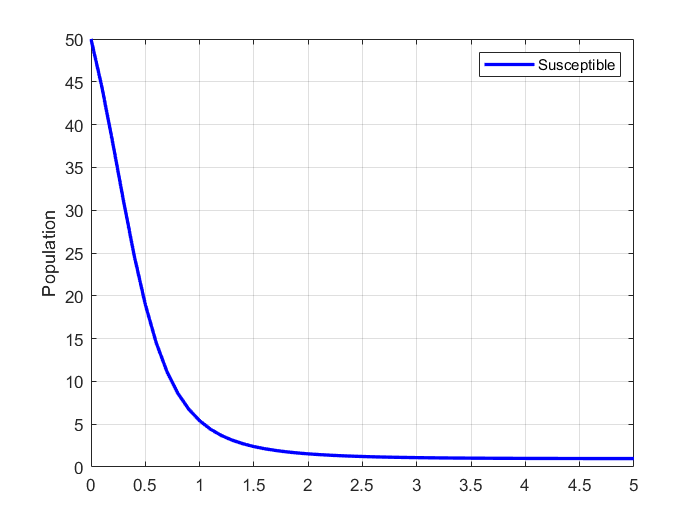
\includegraphics[width=0.5\textwidth]{images/fig_5.png}\label{fig:RK4_22}}
  \caption{Comparison of \(S\) values obtained from the paper's results with our own results  }
\end{figure}

 Example 3: $\alpha=10, r=1 / 10, I_{0}=50, S_{0}=80$

In this case, we have $r S_{0} / \alpha=0.8<1, S_{\infty}=29.19, \beta=7.081$. According to the curve $I_{w} \sim h$ at the 10 th-order of approximation, the HAM series are convergent in the region $-3 \leqslant h<0$. So we choose $h=-2$, and even the second-order HAM series agree well with the numerical ones, as shown in Fig. 6.


\begin{figure}[!htbp]
  \centering
  \subfloat[paper\_result]{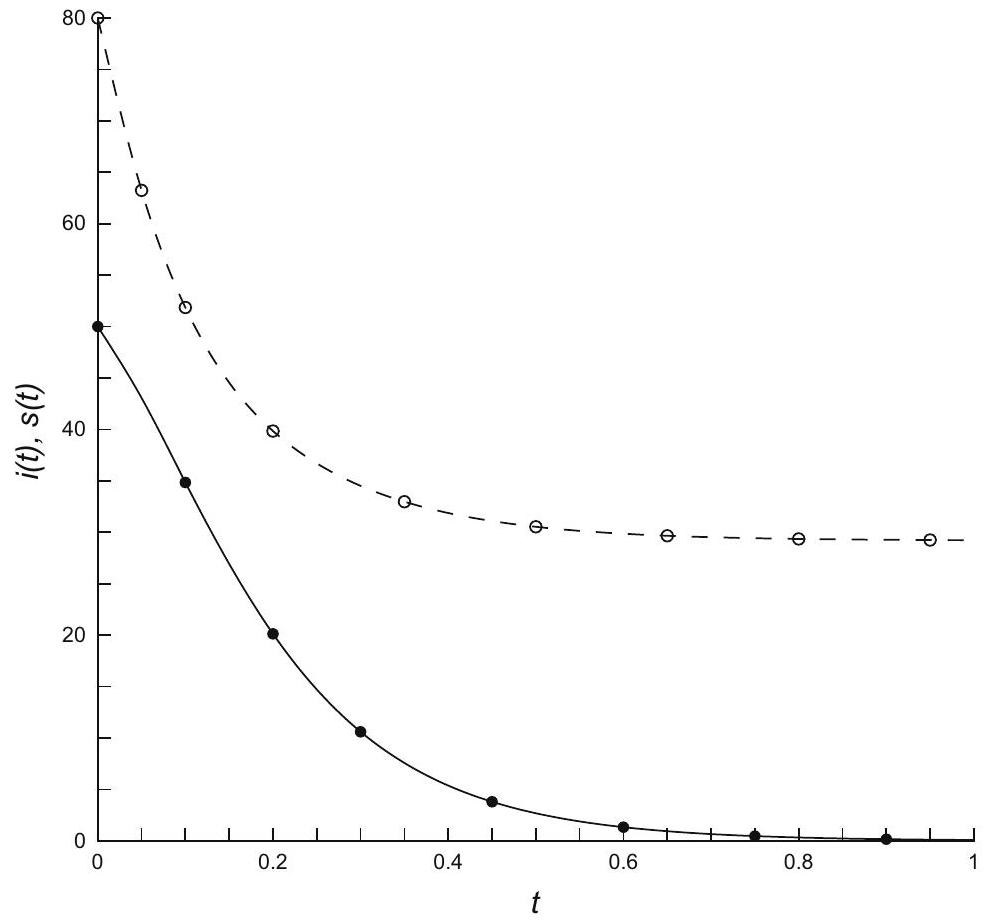
\includegraphics[width=0.5\textwidth]{images/2024_05_06_fa20b94a24cdaf499645g-09(1).jpg}\label{fig:paper_31}}
  \hfill
  \subfloat[own\_result]{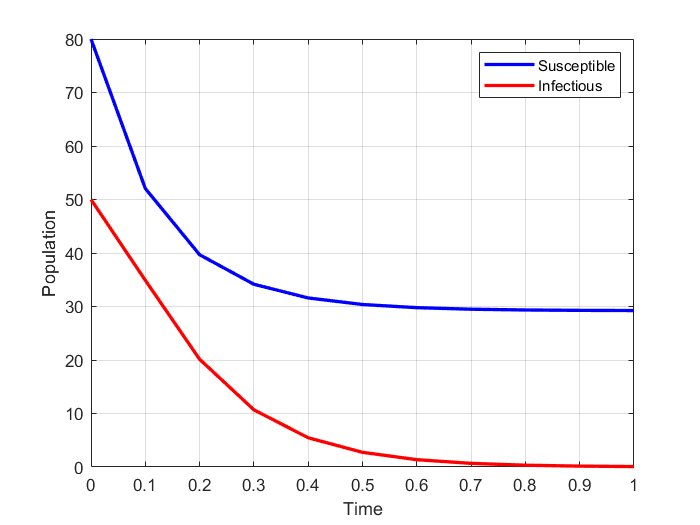
\includegraphics[width=0.5\textwidth]{images/fig_6.png}}\label{fig:RK4_31}
  \caption{Comparison of \(I\)  and \(S\) values obtained from the paper's results with our own results  }
\end{figure}



\subsection*{ Example 4: $\alpha=2.73, r=0.0178, I_{0}=7, S_{0}=254$}
Let us consider a practical case. Over the period from mid-May to mid-October 1966, the village of Eyam in England suffered an outbreak of bubonic plague. The community was asked to quarantine itself so that the disease could be prevented from spreading to other communities. A thorough record was kept according to which it is believed that out of an initial population of 350 persons only 83 survived the Eyam plague. The disease in Eyam has been used as a case study for the basic SIR modeling. Here we try to fit the basic SIR model, measuring time in months with an initial population of 7 infectives and 254 susceptibles and a final population of 83 .
In this case, we have $r S_{0} / \alpha=1.656>1, S_{\infty}=76.05

Now we can see this is matching from our figure with paper figure.


\begin{figure}[!htbp]
  \centering
  \subfloat[paper\_result]{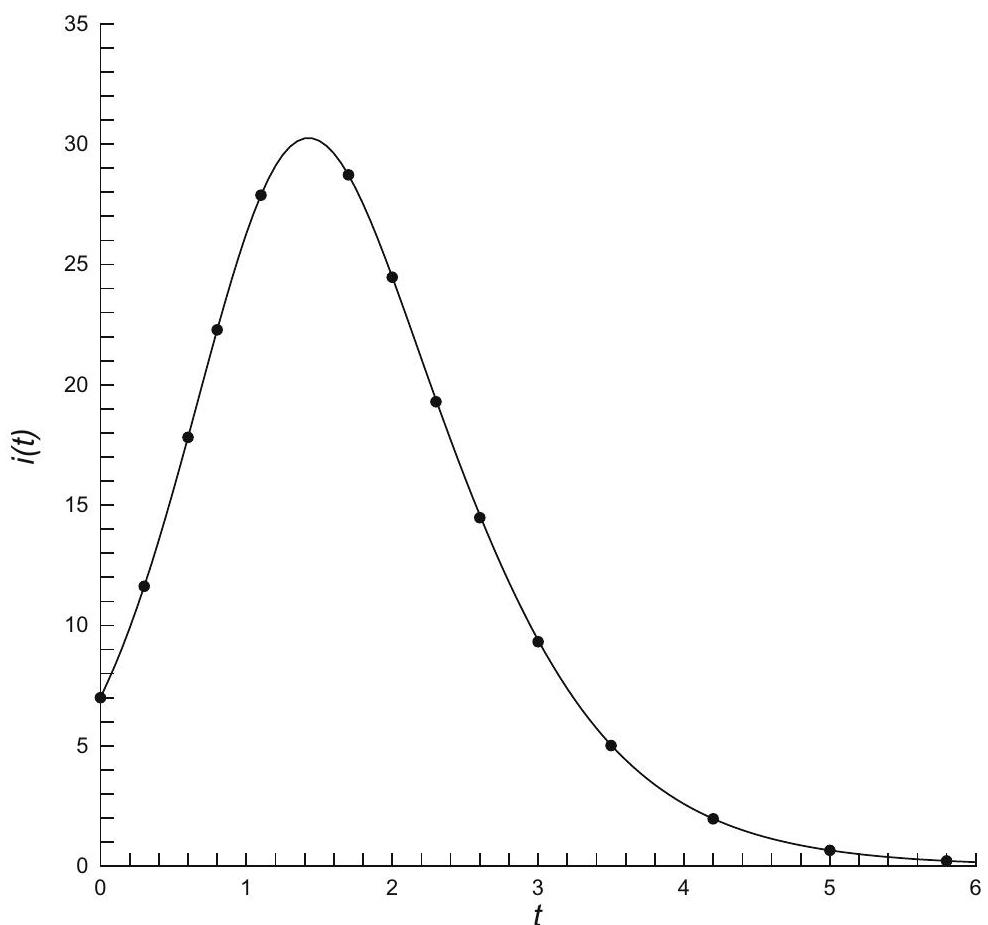
\includegraphics[width=0.5\textwidth]{images/2024_05_06_fa20b94a24cdaf499645g-09.jpg}\label{fig:paper_41}}
  \hfill
  \subfloat[own\_result]{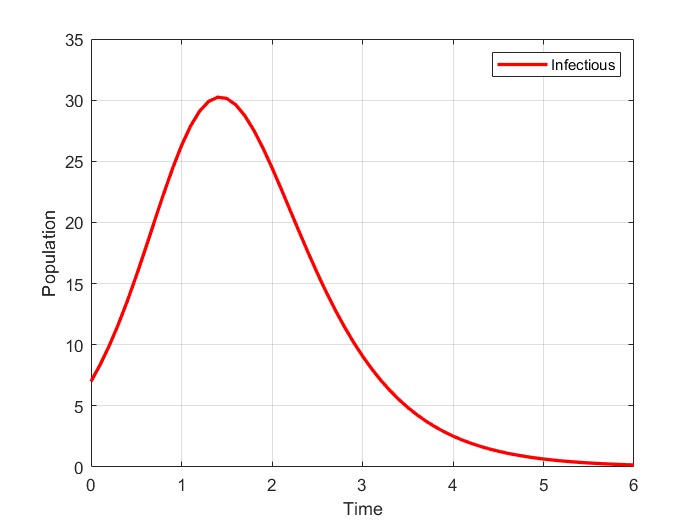
\includegraphics[width=0.5\textwidth]{images/fig_7.png}}\label{fig:RK4_41}
  \caption{Comparison of \(I\) values obtained from the paper's results with our own results  }
\end{figure}
\begin{figure}[!htbp]
  \centering
  \subfloat[paper\_result]{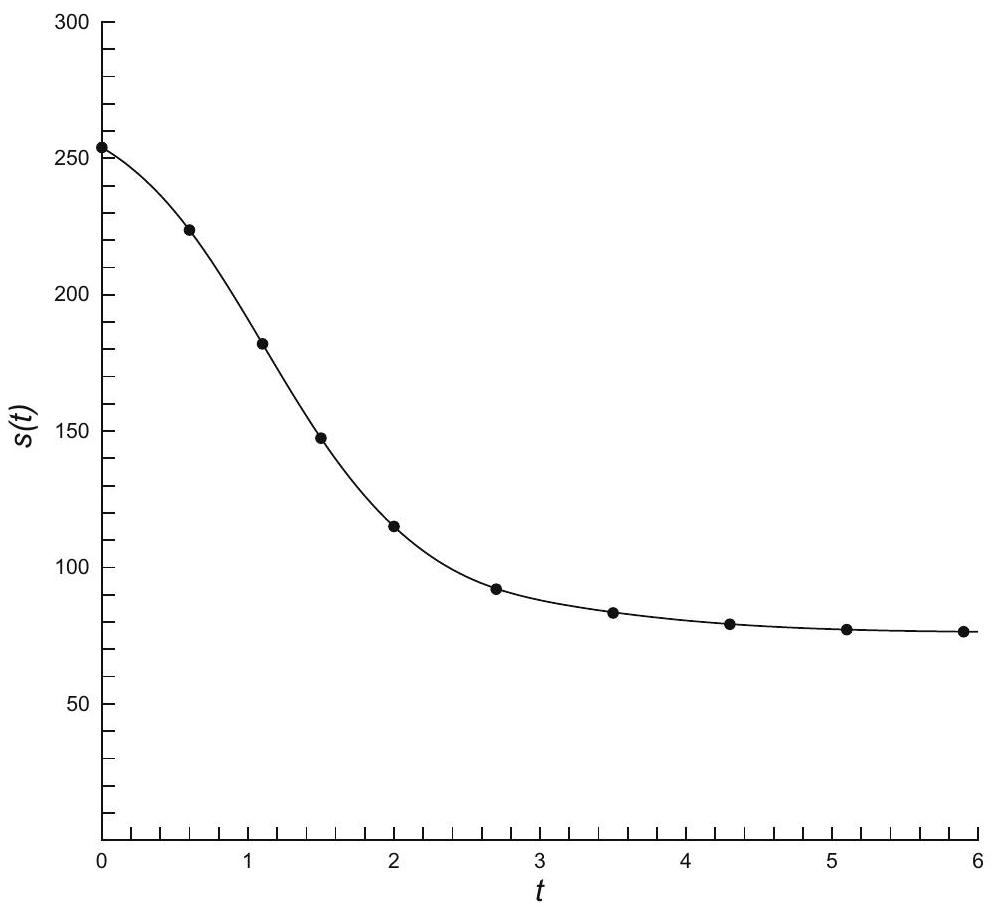
\includegraphics[width=0.5\textwidth]{images/2024_05_06_fa20b94a24cdaf499645g-10.jpg}\label{fig:paper_42}}
  \hfill
  \subfloat[own\_result]{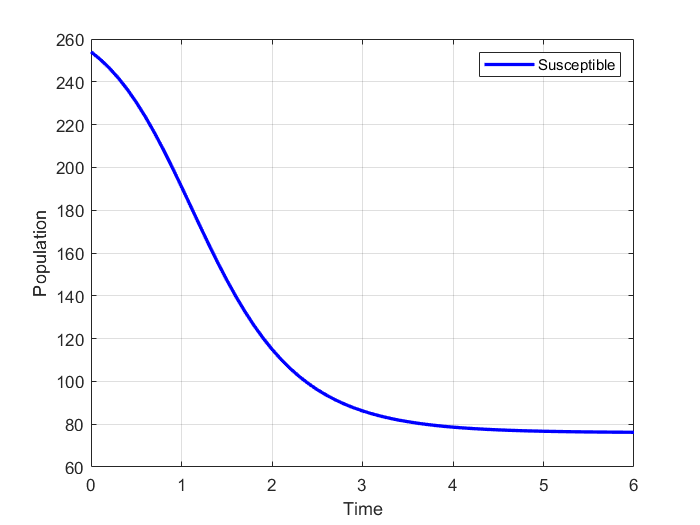
\includegraphics[width=0.5\textwidth]{images/fig_8.png}\label{fig:RK4_42}}
  \caption{Comparison of \(S\) values obtained from the paper's results with our own results  }
\end{figure}
\newpage

\section*{4. RK4 method for  SIS model}
The basic SIS model [1] is given by







\begin{align*}
& s^{\prime}(t)=-r s(t) i(t)+\gamma i(t)  \tag{47}\\
& i^{\prime}(t)=r s(t) i(t)-\gamma i(t) \tag{48}
\end{align*}


subject to initial conditions,


\begin{equation*}
i(0)=I_{0}, \quad s(0)=S_{0} \tag{49}
\end{equation*}


where $r>0, I_{0}>0$ and $S_{0}>0$. Obviously, $S+I=k$, where $k$ is the total population. From (47) and (48), we obtain the threshold value $r k / \gamma$ for this model. There are two different cases for $t$ approaching $\infty$ :

(A) If $r k / \gamma \leqslant 1$ for any $I_{0}$, then




\begin{equation*}
I(+\infty)=0, \quad S(\infty)=k \tag{50}
\end{equation*}
verify with our code
  \begin{center}
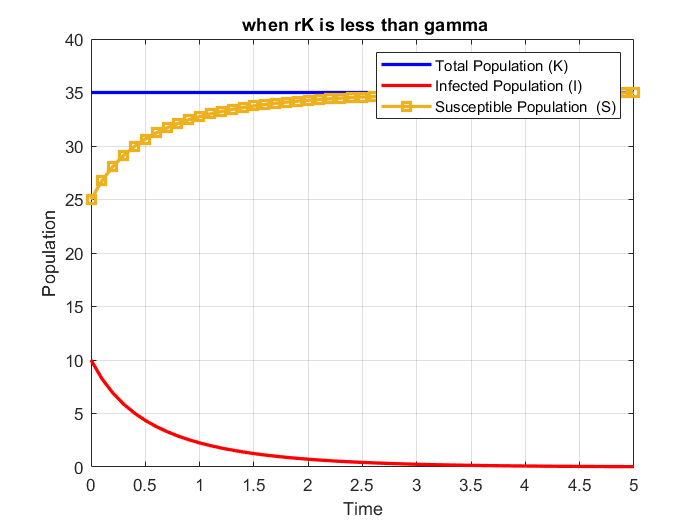
\includegraphics[max width=\textwidth]{images/when_rK_is_less_than_gamma.png}
\end{center}
\newpage
(B)if $r k / \gamma>1$ for any $I_{0}$, then


\begin{equation*}
I(+\infty)=k-\gamma / r, \quad S(+\infty)=\gamma / r \tag{51}
\end{equation*}
verify with our code
  \begin{center}
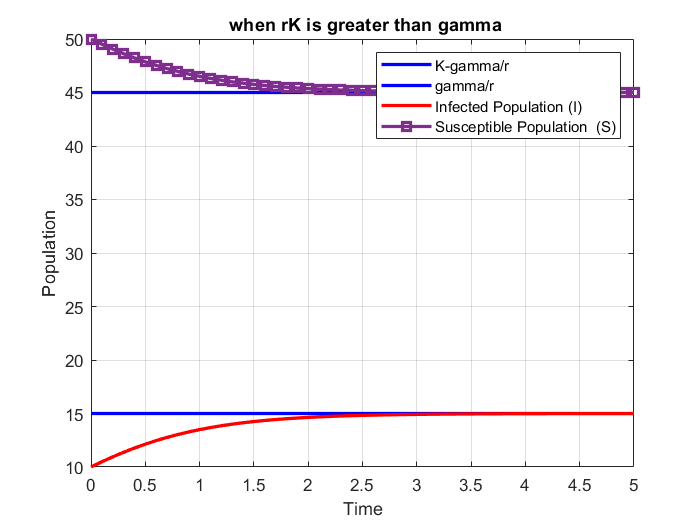
\includegraphics[max width=\textwidth]{images/when_rK_is_greater_than_gamma.png}
\end{center}

Hence, if $r k / \gamma<1$, the infection must vanish, whereas if $r k / \gamma>1$, the infection continues. So the interesting case is $r k / \gamma>1$, the epidemic case. This model is different from the SIR model, because the recovered members return to the class $S$ at a rate of $\gamma i$ instead of moving to class $R$, where $\gamma$ is the recovery coefficient.
\subsection*{3.3.
Solution analysis for the SIS model with examples}

For the SIS model Here we present a few examples of comparison of our RK4 method  solutions of the SIS model with paper results.

\vspace{2\baselineskip}

 Example 5: $\gamma=3 / 2, \beta=2, r=1 / 10, I_{0}=10$ and $S_{0}=25$
  
  In this case we have $r k / \gamma=2.33>1$. So, using (51), we have $S_{\infty}=15$ and $I_{\infty}=20$. Similarly, according to the curve $I_{w} \sim h$ at the 10th-order approximation, The HAM series are convergent for $-2.5 \leqslant h<0$. Choosing $h=-1 / 2$, our explicit series solution agree well with numerical ones, as shown in Figs. (9) and (10).\begin{figure}[htbp]
  \centering
  \subfloat[paper\_result]{\includegraphics[width=0.4\textwidth]{images/2024_05_07_79dc20a88ff3ef7ad507g-13(1).jpg}\label{fig:paper_52}}
  \hfill
  \subfloat[own\_result]{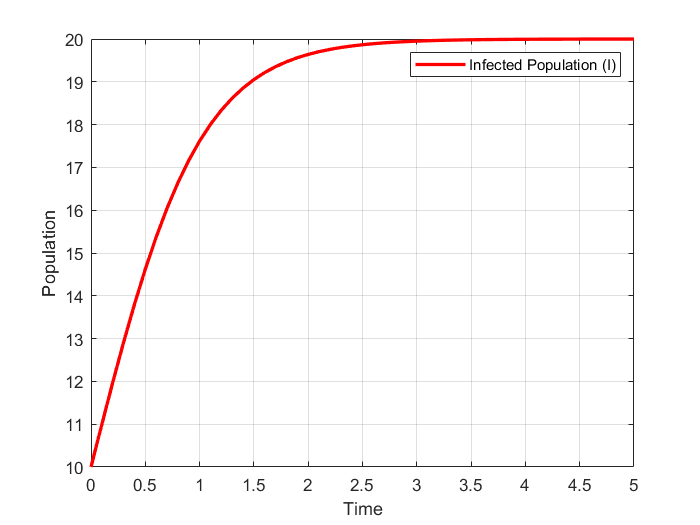
\includegraphics[width=0.5\textwidth]{images/ex_5i.png}\label{fig:RK4_52}}
  \caption{Comparison of \(I\) values obtained from the paper's results with our own results  }
  \end{figure}
  \begin{figure}[htbp]
  \centering
  \subfloat[paper\_result]{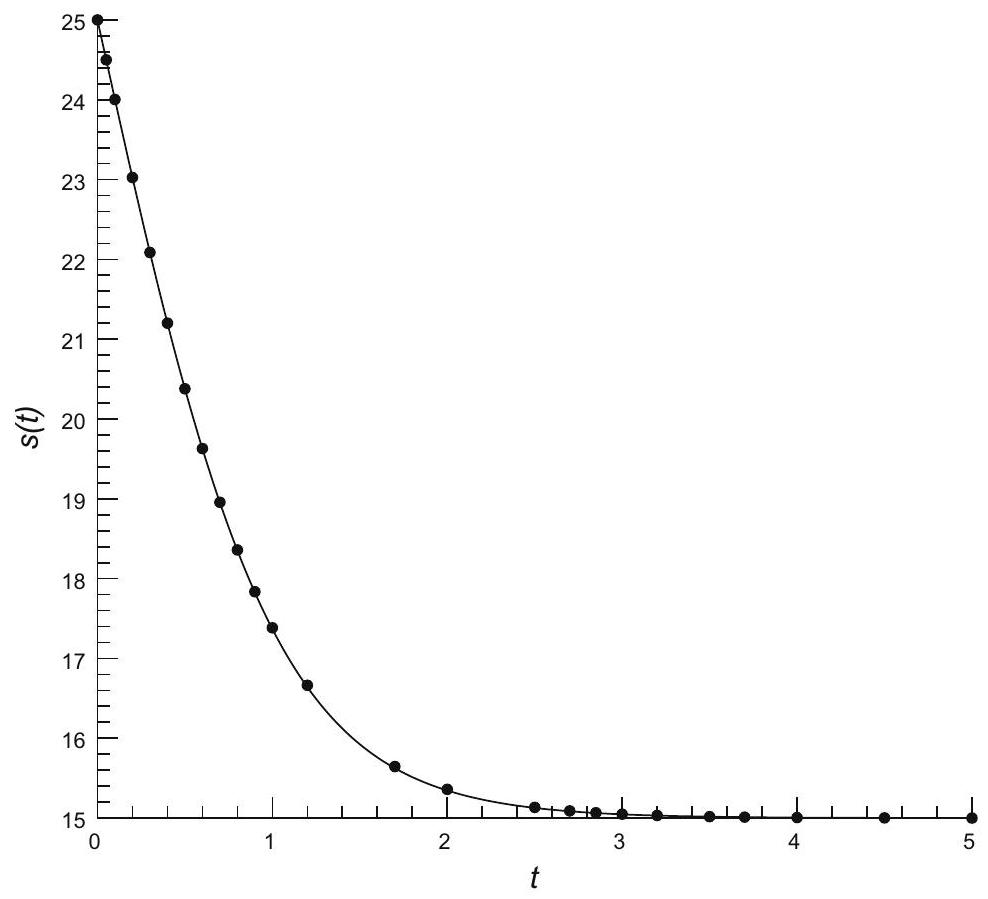
\includegraphics[width=0.4\textwidth]{images/2024_05_07_79dc20a88ff3ef7ad507g-13.jpg}\label{fig:paper_51}}
  \hfill
  \subfloat[own\_result]{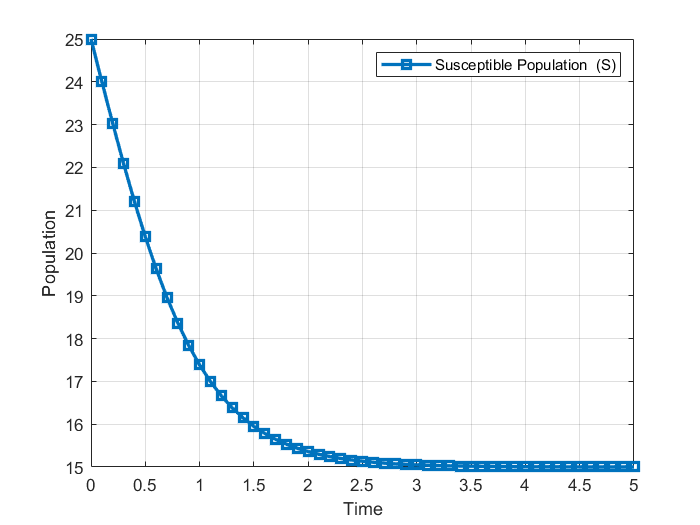
\includegraphics[width=0.5\textwidth]{images/ex_5s.png}\label{fig:RK4_51}}
  \caption{Comparison of \(S\) values obtained from the paper's results with our own results  }
   \end{figure}
\newpage
Example 6: $\gamma=1 / 10, \beta=1, r=1 / 15, I(0)=25$ and $S(0)=10$
This is an example of epidemic because of $r k / \gamma>1$.  HAM series are convergent for $-2 \leqslant h \leqslant 0$. Choosing $h=-1 / 2$, The HAM series solution agree well with the numerical ones.
\begin{figure}[!htbp]
  \centering
  \subfloat[paper\_result]{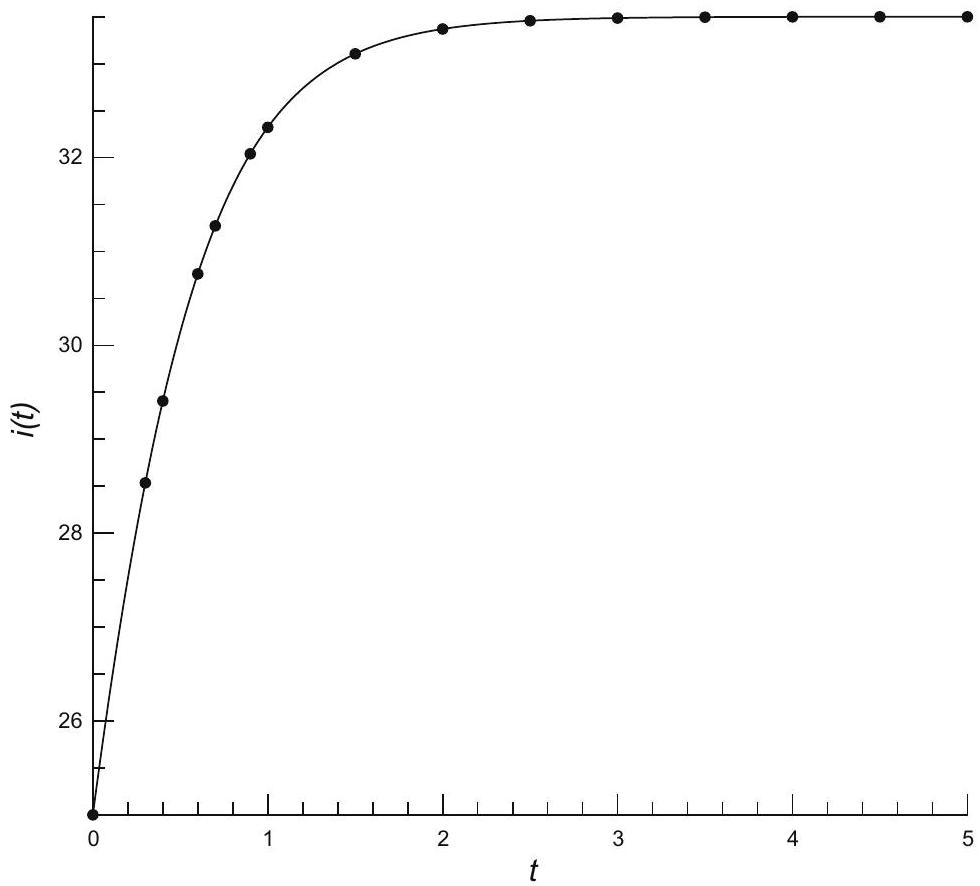
\includegraphics[width=0.4\textwidth]{images/2024_05_07_79dc20a88ff3ef7ad507g-14.jpg}\label{fig:paper_62}}
  \hfill
  \subfloat[own\_result]{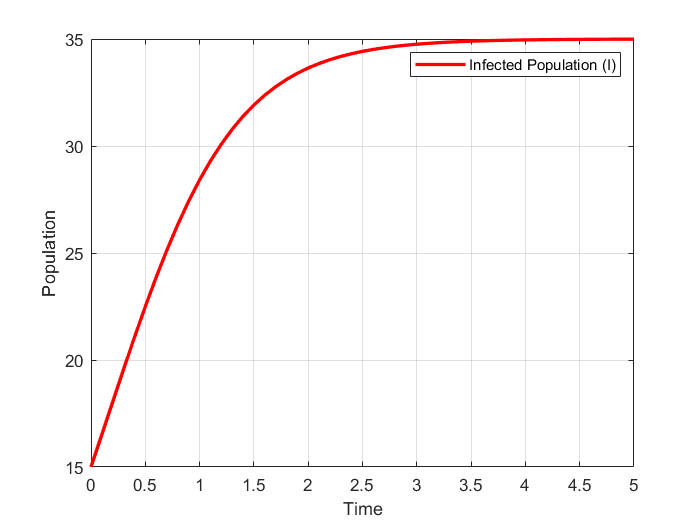
\includegraphics[width=0.5\textwidth]{images/fig_11.png}\label{fig:RK4_62}}
  \caption{Comparison of \(I\) values obtained from the paper's results with our own results  }
\end{figure}
\begin{figure}[!htbp]
  \centering
  \subfloat[paper\_result]{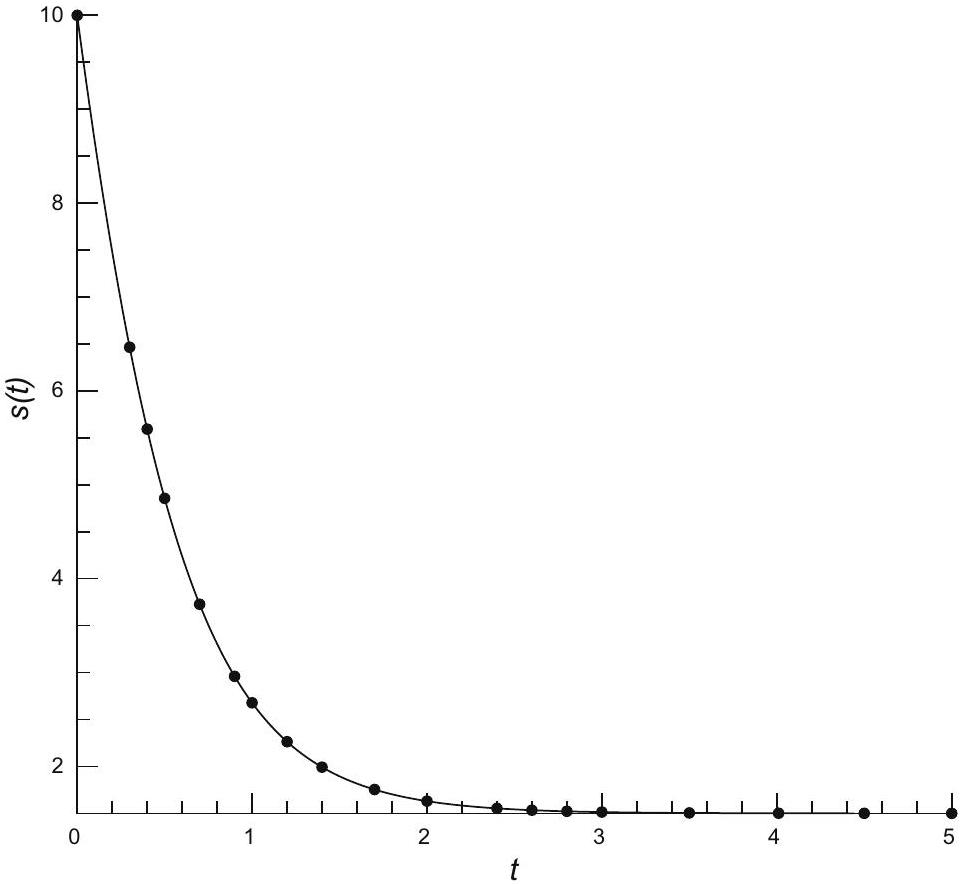
\includegraphics[width=0.4\textwidth]{images/2024_05_07_79dc20a88ff3ef7ad507g-14(1).jpg}\label{fig:paper_61}}
  \hfill
  \subfloat[own\_result]{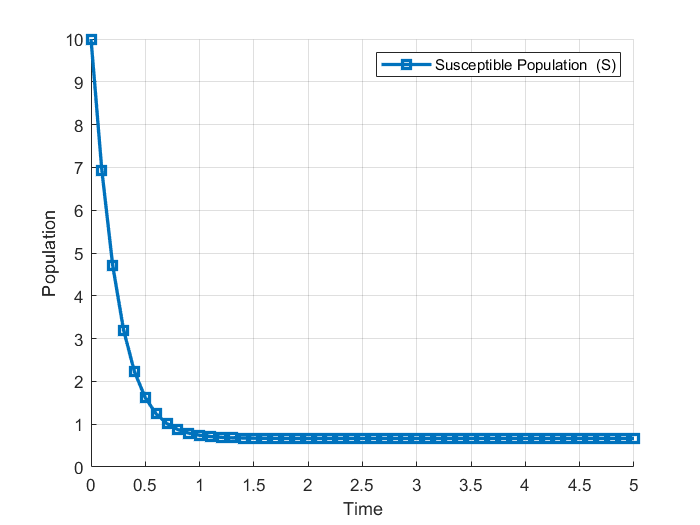
\includegraphics[width=0.5\textwidth]{images/fig_12.png}\label{fig:RK4_61}}
  \caption{Comparison of \(S\) values obtained from the paper's results with our own results  }
\end{figure}


3.3.3. Example 7: $\gamma=3 / 2, \beta=1, r=1 / 20, I(0)=15$ and $S(0)=50$
 \begin{figure}[!htbp]
  \centering
  \subfloat[paper\_result]{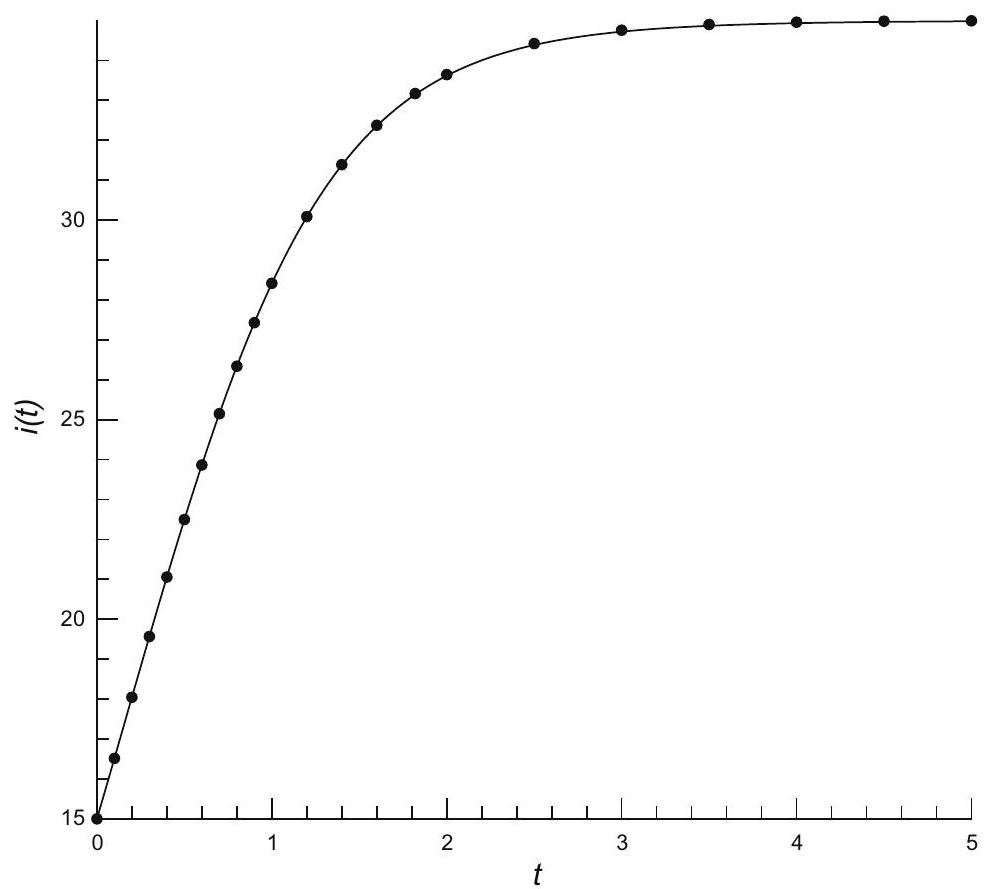
\includegraphics[width=0.4\textwidth]{images/2024_05_07_79dc20a88ff3ef7ad507g-15(1).jpg}\label{fig:paper_72}}
  \hfill
  \subfloat[own\_result]{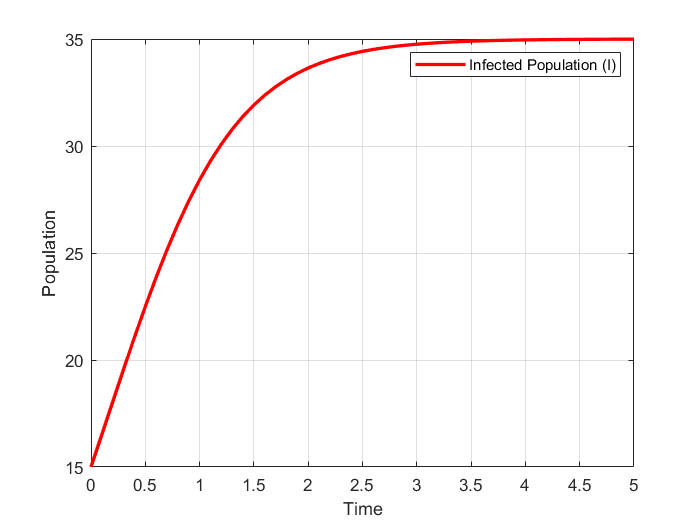
\includegraphics[width=0.5\textwidth]{images/fig_13.png}\label{fig:RK4_72}}
  \caption{Comparison of \(I\) values obtained from the paper's results with our own results  }
\end{figure}
\begin{figure}[!htbp]
  \centering
  \subfloat[paper\_result]{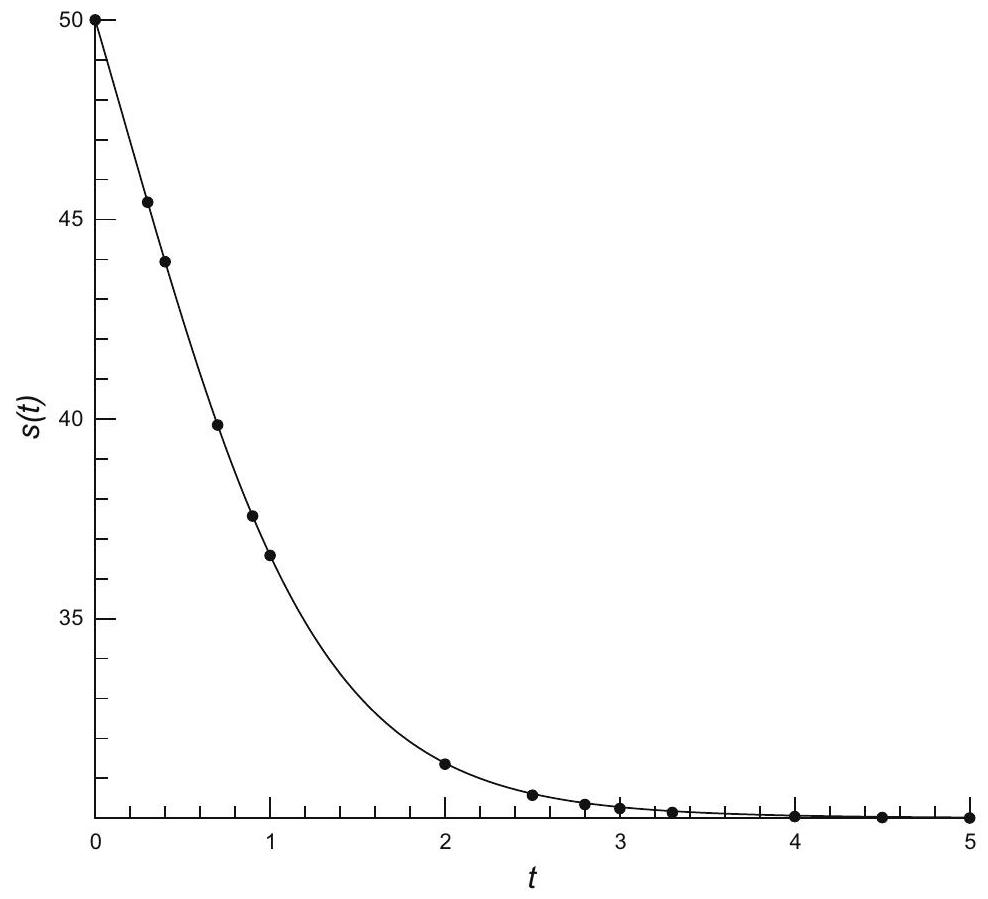
\includegraphics[width=0.4\textwidth]{images/2024_05_07_79dc20a88ff3ef7ad507g-15.jpg}\label{fig:paper_71}}
  \hfill
  \subfloat[own\_result]{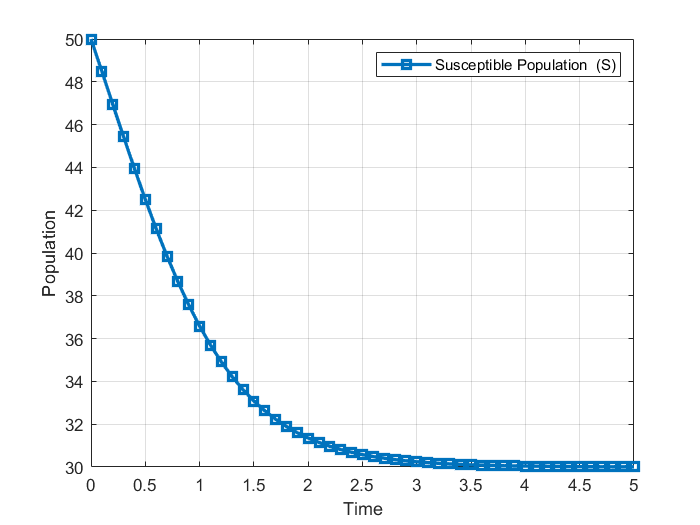
\includegraphics[width=0.5\textwidth]{images/fig_14.png}\label{fig:RK4_71}}
  \caption{Comparison of \(S\) values obtained from the paper's results with our own results  }
\end{figure}
Similarly, it is found that the  HAM series are convergent for $-3 \leqslant h<0$. Choosing $h=-2 / 5$, the HAM series solution agree well with numerical ones, as shown in Figs. (13) and (14). This is also an example of epidemic for $r k / \gamma>1$.

\begin{center}
\includegraphics[max width=\textwidth]{2024_05_07_79dc20a88ff3ef7ad507g-13(1)}
\end{center}
\newpage


3.3.4. Example 8 : $\gamma=2, \beta=1, r=1 / 20, I(0)=5, S(0)=15$

In this example we have $r k / \gamma=0.5<1$ which shows no epidemic. 


\begin{figure}[!htbp]
  \centering
  \subfloat[paper\_result]{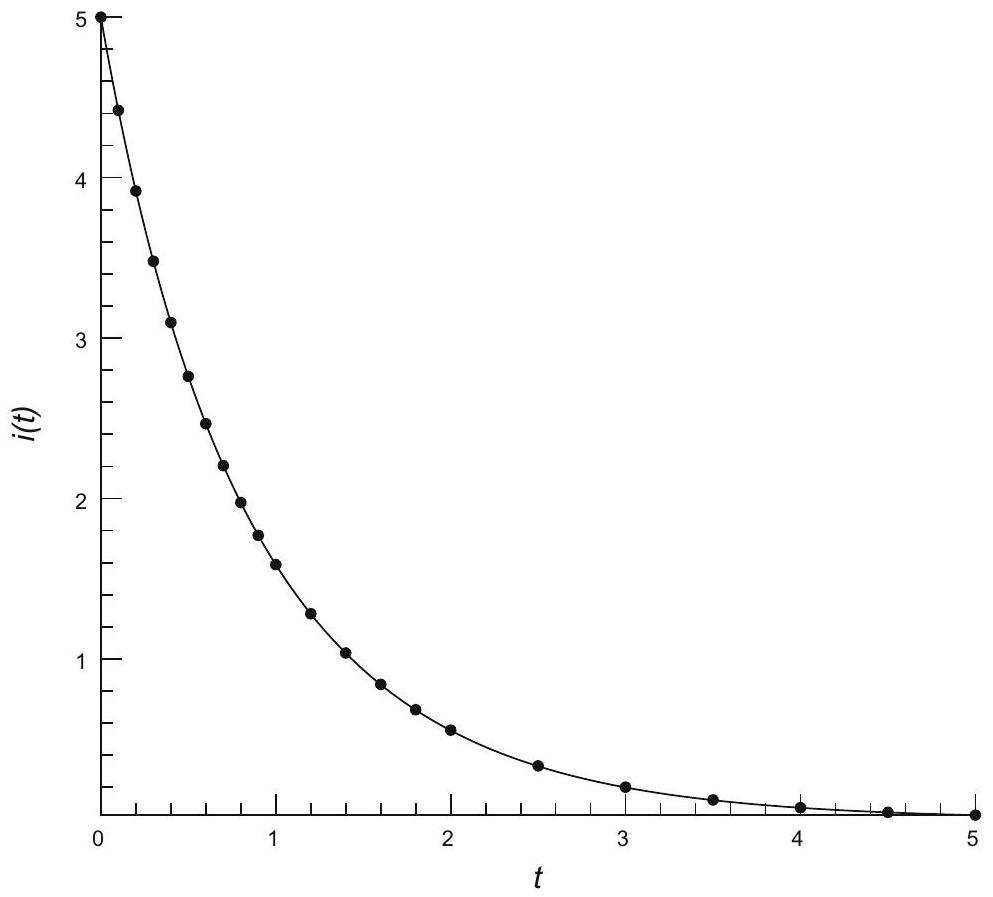
\includegraphics[width=0.4\textwidth]{images/2024_05_07_79dc20a88ff3ef7ad507g-16.jpg}\label{fig:paper_92}}
  \hfill
  \subfloat[own\_result]{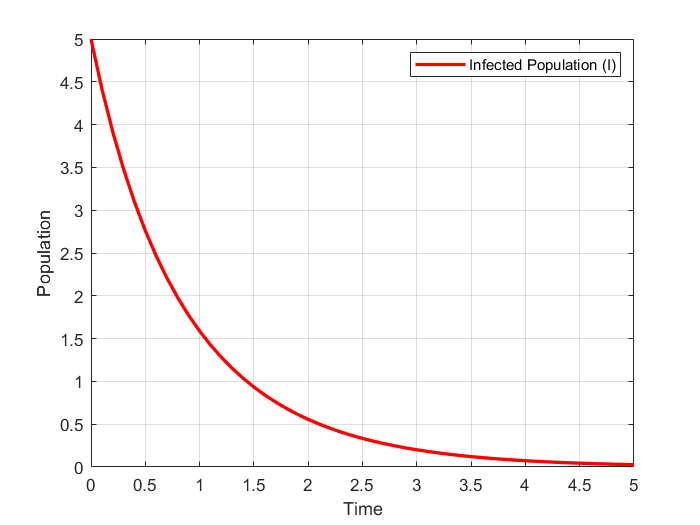
\includegraphics[width=0.5\textwidth]{images/fig_15.png}\label{fig:RK4_42}}
  \caption{Comparison of \(I\) values obtained from the paper's results with our own results  }
\end{figure}

\begin{figure}[!htbp]
  \centering
  \subfloat[paper\_result]{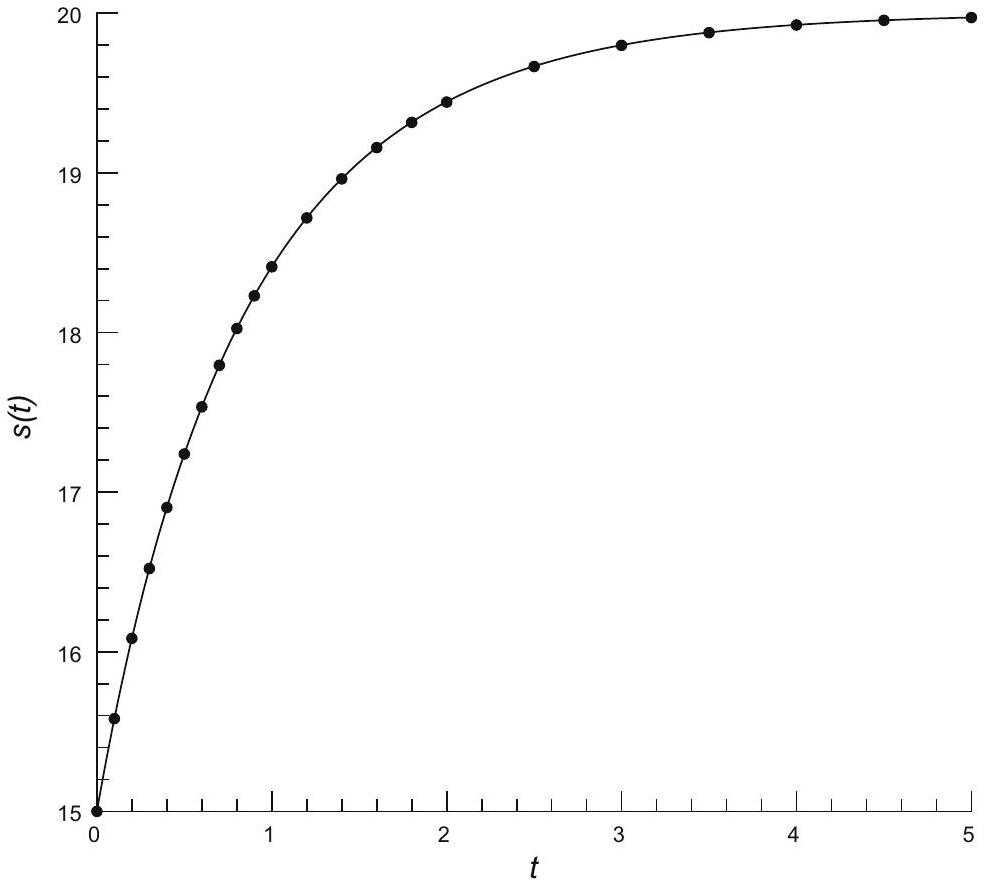
\includegraphics[width=0.4\textwidth]{images/2024_05_07_79dc20a88ff3ef7ad507g-16(1).jpg}\label{fig:paper_92}}
  \hfill
  \subfloat[own\_result]{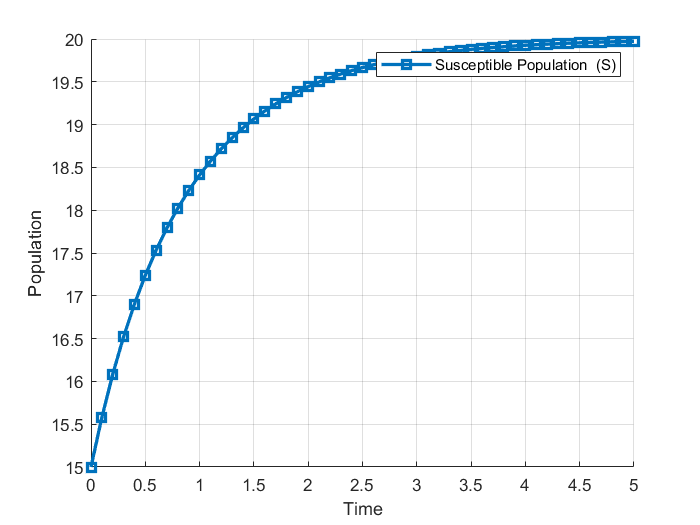
\includegraphics[width=0.5\textwidth]{images/fig_16.png}\label{fig:RK4_42}}
  \caption{Comparison of \(S\) values obtained from the paper's results with our own results  }
\end{figure}
\newpage
All of these examples show the validity of our RK4 method solutions for the SIR and SIS models.

\section*{5. Conclusion}
In this report, the SIR and SIS models, commonly used in epidemiology, are solved using the fourth-order Runge-Kutta (RK4) method. By discretizing the original nonlinear differential equations into a series of linear subproblems, RK4 computes numerical solutions that closely match analytical results. The use of RK4 provides efficient and accurate solutions for these models.

\end{document}